% ============================================================
% CascadeBench — SoftwareX Original Software Publication
% Class: elsarticle (SoftwareX template). Compile:
%   pdflatex main ; bibtex main ; pdflatex main ; pdflatex main
% On Overleaf: set this file as the main document (elsarticle ships with TeX Live).
% ============================================================
\documentclass[final,5p,times]{elsarticle}

\usepackage[T1]{fontenc}
\usepackage[utf8]{inputenc}
\usepackage{amsmath,amssymb}
\usepackage{booktabs}
\usepackage{multirow}
\usepackage{array}
\usepackage{tabularx}
\usepackage{float}
\usepackage{graphicx}
\usepackage{xcolor}
\usepackage{listings}
\usepackage{enumitem}
\usepackage{tikz}
\usetikzlibrary{arrows.meta,positioning,fit,backgrounds}
\usepackage{xspace}
\usepackage{hyperref}

\lstset{
  basicstyle=\ttfamily\footnotesize,
  breaklines=true,
  columns=fullflexible,
  keepspaces=true,
  frame=single,
  framesep=4pt,
  xleftmargin=4pt,
  showstringspaces=false,
  language=Python
}

\newcommand{\tool}{CascadeBench\xspace}

\journal{SoftwareX}

\begin{document}

\begin{frontmatter}

\title{CascadeBench: A Leak-Aware Benchmark for Graph-Based\\
Spear-Phishing and Lateral-Movement Detection}

\author[koz]{Kamil Warpechowski\corref{cor}}
\ead{kamil.warpechowski@kozminski.edu.pl}
\author[koz,nask]{Bogdan Ksi\k{e}\.zopolski}
\ead{bogdan.ksiezopolski@kozminski.edu.pl}

\address[koz]{Kozminski University, Jagiello\'nska 57/59, 03-301 Warsaw, Poland}
\address[nask]{NASK National Research Institute, Warsaw, Poland}
\cortext[cor]{Corresponding author.}

\begin{abstract}
\noindent
Graph-based detectors of spear phishing, business email compromise, and lateral movement are
evaluated on private corpora saturated with confounders---rhythm, degree, volume, and
identity leakage---so reported scores reflect artefacts, not the attack mechanism.
\emph{CascadeBench} is an installable Python toolkit that makes such evaluation controllable
and reproducible: it builds communication graphs (synthetic, SNAP, Enron), injects a
programmable cascade attacker that trades reach against evasion with ground-truth labels, and
scores a detector panel under a \emph{leak-aware} protocol---matched-design benign traffic,
victim-disjoint splits, a time-shuffle causality control, and operational Recall@low-FPR
metrics. One interface lets researchers plug in new graphs, attacks, and detectors, turning
confounder-prone results into a shared, falsifiable benchmark.
\end{abstract}

\begin{keyword}
spear phishing \sep lateral movement \sep graph neural networks \sep
adversarial evaluation \sep benchmark \sep data leakage
\end{keyword}

\end{frontmatter}

\section{Motivation and significance}
\label{sec:intro}

Mass phishing is, for practical purposes, a solved filtering problem: modern email security
intercepts the overwhelming majority of bulk campaigns. The residual, disproportionately
costly threat is \emph{targeted}---spear phishing, business email compromise (BEC), and
lateral phishing sent from an already-compromised internal account
\cite{ho2019detecting,cidon2019high,apwg2024trends}. These messages are hard precisely
because they are \emph{contextually legitimate}: the sender is a plausible or genuine
contact, the timing is unremarkable, and the request often continues a real thread. They
carry no malware and little lexical anomaly, so content-only classifiers degrade toward
chance on exactly the cases that inflict the largest losses.

A natural response is to stop looking only at the message and start looking at the
\emph{relations} around it. If one models an organization's communication as a graph---who
talks to whom, when, and through which channel---then a targeted attack becomes a structural
or temporal irregularity: an edge that should not exist, a sender whose neighbourhood
behaviour shifts, a burst that violates the local rhythm. This intuition has driven a decade
of work, from account-compromise heuristics \cite{egele2013compa,stringhini2015thataint}
and lateral-phishing feature models \cite{ho2019detecting} to graph neural networks (GNNs)
\cite{kipf2017semisupervised,hamilton2017inductive} adapted from fraud and anomaly detection
\cite{dou2020enhancing,ma2021comprehensive}.

\paragraph{The problem: evaluation, not models.} What the field lacks is not another model
but a way to \emph{believe} the numbers. Real lateral-phishing corpora are proprietary,
small, and saturated with confounders. Attacker events systematically differ from benign
events in send-time rhythm (off-hours activity), sender degree (unusual recipient sets),
volume, and identity (a few repeated malicious senders). A detector can therefore achieve a
high score by keying on these artefacts rather than on the mechanism of the attack---and
such a detector fails on a new tenant or after the attacker adapts. This is the security-ML
measurement trap documented broadly by \citet{arp2022dos} and quantified for temporal drift
by \citet{pendlebury2019tesseract}. In the graph setting the risk is acute: node degree and
timing are exactly the features a GNN will happily overfit. No open, reusable testbed today
offers, simultaneously, (i) ground-truth labels, (ii) a controllable \emph{adaptive}
attacker, and (iii) explicit leakage controls. As a result, published results are point AUCs
on incomparable private data, and it is impossible to tell mechanism from confounder.

\paragraph{Contributions.} We address this with \tool, an installable, extensible toolkit
for adversarial, leakage-controlled evaluation of graph-based phishing and lateral-movement
detectors. Concretely:

\begin{itemize}[leftmargin=1.4em,itemsep=2pt]
\item \textbf{A controllable testbed} coupling three graph sources (a procedural
  organization model, SNAP email networks \cite{leskovec2014snap}, and the Enron corpus
  \cite{klimt2004enron}) with a programmable \emph{cascade} attacker whose reach/evasion
  trade-off is a small set of parameters, producing scenarios with per-event ground truth
  (Section~\ref{sec:method}).
\item \textbf{A leak-aware evaluation protocol}---benign traffic matched by design to the
  attack's endpoint and degree distribution, victim-disjoint splits, a time-shuffle
  causality control, and operational Recall@low-FPR metrics---that separates the attack
  mechanism from the four confounders above (Section~\ref{sec:method}).
\item \textbf{A detector panel behind one interface}, spanning tabular baselines,
  account-compromise heuristics, an anomaly forest, and static/temporal GNNs, so that
  heterogeneous methods are compared on identical, audited footing.
\item \textbf{An automatic red/blue arms-race} that co-searches attack and defense spaces to
  produce robustness frontiers rather than single-point scores.
\item \textbf{An open, GDPR-free artefact}: the synthetic population contains no personal
  data, and all experiments reproduce offline from bundled result files.
\end{itemize}

\paragraph{Analyses the tool supports.} \tool operationalizes analyses that closed corpora
cannot, which the authors' companion studies on graph-based spear-phishing detection (in
preparation) rely on: \textbf{(A1)} which graph structures carry signal for which attack type;
\textbf{(A2)} whether a detector's advantage survives a time-shuffle---mechanism or leakage;
\textbf{(A3)} how detection degrades as an attacker trades reach for evasion; and
\textbf{(A4)} whether a detector's robustness transfers across conditions. This paper describes
the \emph{software} that makes such analyses reproducible; the corresponding scientific results
and their interpretation are reported separately. Section~\ref{sec:related} positions the tool
against detection methods and evaluation critiques; Section~\ref{sec:method} describes the
software; Section~\ref{sec:results} gives illustrative examples;
Section~\ref{sec:discussion} details impact and limitations;
Section~\ref{sec:conclusion} concludes.
\subsection{Related work}
\label{sec:related}

\subsubsection{Detecting targeted email attacks}
Early defenses against account compromise keyed on behavioural profiles: COMPA
\cite{egele2013compa} flags messages that deviate from a per-account statistical model, and
\citet{stringhini2015thataint} block spearphishing by modelling each sender's habitual
behaviour and raising an alert when a message does not match it. A parallel line detects
spear phishing \emph{content-agnostically}, from email header and stylometric features
\cite{duman2016emailprofiler} to transport- and behaviour-level traits
\cite{gascon2018reading}, motivated by human-factors studies showing why targeted lures
succeed \cite{halevi2015spearphishing}. For enterprise email specifically,
\citet{ho2019detecting} characterize lateral phishing at scale, \citet{cidon2019high} target
BEC with high-precision content and metadata signals, and \citet{ho2021hopper} model lateral
\emph{movement} as suspicious login/access paths---directly inspiring our Hopper-style
detector. More recent work applies GNNs to phishing email graphs \cite{safran2025phishinggnn}.
These systems establish that relational and behavioural context is discriminative, but each is
validated on a single proprietary corpus, so their reported operating points are not directly
comparable---the gap \tool addresses.

\subsubsection{Graph and GNN approaches}
Graph neural networks---graph convolution \cite{kipf2017semisupervised}, inductive
neighbourhood sampling \cite{hamilton2017inductive}, and attention
\cite{velickovic2018graph}---are the default tool for relational anomaly and fraud detection,
with known limits on expressive power \cite{xu2019how} and large surveys of the design space
\cite{wu2021comprehensive,ma2021comprehensive,akoglu2015graph}. For fraud specifically, a
recurring finding is that fraudsters \emph{camouflage} by attaching to benign neighbourhoods,
which motivates label-imbalance- and camouflage-robust detectors
\cite{dou2020enhancing,liu2021pick,tang2022rethinking} and large public graph-fraud benchmarks
\cite{weber2019antimoney}. Because email is a \emph{dynamic} graph, temporal architectures are
a natural fit: temporal graph networks \cite{rossi2020temporal}, temporal attention
\cite{xu2020inductive}, and evolving GCNs \cite{pareja2020evolvegcn}. Finally, GNNs are
themselves attackable through adversarial edges \cite{zugner2018adversarial}, with defenses
such as \cite{zhang2020gnnguard}---exactly the adversarial regime \tool is built to probe. Our
detector panel deliberately spans this range---tabular baselines, an account-compromise
heuristic, an anomaly forest, a static GCN, and temporal GNNs with and without attention---so
that architectural choices are compared on identical footing rather than across papers.

\subsubsection{Evaluation pitfalls and the missing testbed}
A parallel literature warns that security-ML results are frequently optimistic.
\citet{arp2022dos} catalogue pervasive pitfalls---sampling bias, spurious correlations,
inappropriate baselines---and \citet{pendlebury2019tesseract} show that ignoring temporal
and spatial bias inflates malware-classification metrics that then collapse under realistic
deployment. In the graph setting these hazards are sharpened: node degree, send-time, and a
small set of repeated malicious identities are exactly the shortcuts a model will exploit.
Despite this, phishing and lateral-movement detectors are still typically evaluated on
closed corpora without leakage controls, matched benign designs, or operational metrics.
There is, to our knowledge, no open, reusable testbed that supplies ground-truth labels, an
adaptive attacker, and explicit confounder controls together. \tool is designed to be
exactly that instrument: it does not propose a new detector but makes the comparison of
existing and future detectors credible and reproducible.
\section{Software description}
\label{sec:method}

\tool is a pure-Python package (\texttt{cascadebench}) exposing both a library API and a
command-line interface. It depends only on NumPy, scikit-learn, LightGBM
\cite{ke2017lightgbm}, and PyTorch; a CPU is sufficient, and a GPU only accelerates the GNN
detectors. This section describes the architecture, the graph and attacker models, the
detector panel, and the leak-aware evaluation protocol that is the tool's core contribution.

\subsection{Architecture}
The toolkit is a five-stage pipeline (Fig.~\ref{fig:arch}). Each stage is an independent,
replaceable component that communicates through typed objects---\texttt{Graph},
\texttt{Scenario}, and \texttt{Detector}---so any single stage can be swapped without
touching the others. This is what turns \tool from a script into a benchmark: a new graph, a
new attack, or a new detector drops into one slot and is immediately measured under the same
protocol.

\begin{figure}[H]
\centering
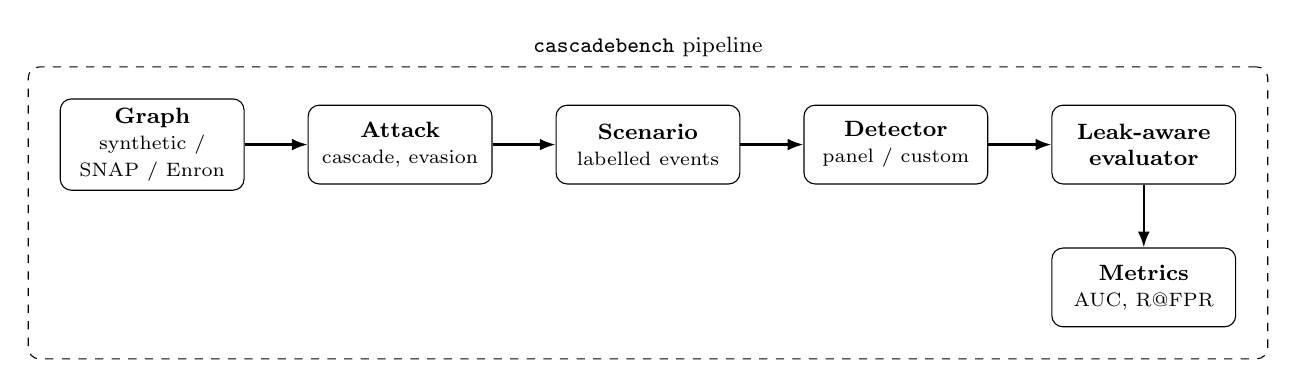
\begin{tikzpicture}[
  node distance=6mm and 8mm,
  box/.style={draw, rounded corners, align=center, minimum height=10mm,
              text width=21mm, font=\footnotesize},
  arr/.style={-{Latex[length=2mm]}, thick}]
  \node[box] (g) {\textbf{Graph}\\\scriptsize synthetic / SNAP / Enron};
  \node[box, right=of g] (a) {\textbf{Attack}\\\scriptsize cascade, evasion};
  \node[box, right=of a] (s) {\textbf{Scenario}\\\scriptsize labelled events};
  \node[box, right=of s] (d) {\textbf{Detector}\\\scriptsize panel / custom};
  \node[box, right=of d] (e) {\textbf{Leak-aware evaluator}};
  \node[box, below=8mm of e] (o) {\textbf{Metrics}\\\scriptsize AUC, R@FPR};
  \draw[arr] (g)--(a); \draw[arr] (a)--(s); \draw[arr] (s)--(d);
  \draw[arr] (d)--(e); \draw[arr] (e)--(o);
  \begin{scope}[on background layer]
    \node[draw, dashed, rounded corners, fit=(g)(a)(s)(d)(e)(o),
          inner sep=4mm, label=above:{\footnotesize\texttt{cascadebench} pipeline}] {};
  \end{scope}
\end{tikzpicture}
\caption{Component architecture. Data flows left to right through replaceable stages; the
evaluator enforces the leakage controls of Section~\ref{sec:leak}.}
\label{fig:arch}
\end{figure}

\subsection{Graph models}
The \texttt{graph} module supplies three sources of communication structure.
\texttt{Graph.synthetic(N)} generates a procedural organization---companies of employees with
internal hierarchy and cross-company partner links---giving full control over topology for
ablations. \texttt{Graph.from\_edgelist} ingests any SNAP-format edge list
\cite{leskovec2014snap} (\texttt{src dst [timestamp]}), and \texttt{load("enron")} loads a
real corporate email graph \cite{klimt2004enron} for external validity. All three expose a
uniform interface (nodes, timestamped edges, and per-node rhythm buckets), so downstream
stages are agnostic to the graph's origin.

\subsection{Attacker model}
The \texttt{attack} module makes the adversary a first-class, programmable object.
\texttt{CascadeStrategy} parameterizes a spreading attack along two axes: \emph{reach}
(\texttt{fanout}, how many recipients a compromised node targets) versus \emph{evasion}
(\texttt{spread}, temporal/structural dispersion; content \texttt{mimicry}; and edge
\texttt{fabrication}, i.e.\ synthesizing plausible OSINT-based contacts). \texttt{cascade}
propagates the attack over the graph and \texttt{build\_scenario} emits a \texttt{Scenario}:
a labelled stream of events with per-event ground truth. Because reach and evasion are
explicit knobs, the same graph yields anything from a loud, wide campaign to a stealthy,
narrow one, and an \emph{adaptive} attacker can be swept to trace how detection degrades as
the adversary invests in evasion.

\subsection{Detector panel}
The \texttt{detect} module provides eight detectors behind a single \texttt{Detector}
interface whose only required method is
\texttt{fit\_score(scenario, train\_mask, test\_mask, seed)}. The panel spans the design
space: a 1-hop tabular baseline and a hand-crafted context model (both backed by LightGBM
\cite{ke2017lightgbm}), the COMPA account-compromise heuristic \cite{egele2013compa}, a
Hopper-style lateral-movement path detector \cite{ho2021hopper}, an isolation-forest anomaly
detector, a static graph convolutional network \cite{kipf2017semisupervised}, and temporal
GNNs with and without attention \cite{rossi2020temporal,xu2020inductive,velickovic2018graph}.
Placing heuristics and GNNs behind one interface is deliberate: it forces every method through
the identical leak-aware protocol, so differences reflect the method, not the harness.

\subsection{Leak-aware evaluation}
\label{sec:leak}
The evaluator (\texttt{evaluate}) is the scientific core. Instead of a single AUC on an
unmatched split, it enforces four controls that separate mechanism from artefact.

\paragraph{(1) Matched-design benign traffic.} Benign events are sampled to match the
attack's endpoint and degree distribution, removing the identity- and degree-based
shortcuts that let a model ``detect'' attacks by recognizing which nodes are involved.

\paragraph{(2) Victim-disjoint splits.} \texttt{victim\_split} guarantees that no victim or
organization appears in both train and test, preventing per-victim memorization---the
graph analogue of the spatial-bias problem of \citet{pendlebury2019tesseract}.

\paragraph{(3) Time-shuffle causality control.} \texttt{shuffle\_time} permutes event
timestamps; a genuine temporal-dynamics signal must vanish under this permutation. A
detector that retains its advantage after shuffling is exploiting a timing confounder, not
the attack, and the tool reports the gap explicitly as a leakage diagnostic.

\paragraph{(4) Operational metrics.} Alongside AUC, the evaluator reports Recall at fixed
low false-positive rates. For a score threshold $\tau$ and false-positive rate
$\mathrm{FPR}(\tau)=\frac{|\{\text{benign}: s>\tau\}|}{|\text{benign}|}$, we report
\[
  \mathrm{Recall@}\alpha \;=\; \mathrm{TPR}\!\big(\tau_\alpha\big),\qquad
  \tau_\alpha=\min\{\tau:\mathrm{FPR}(\tau)\le\alpha\},
\]
for $\alpha\in\{0.1\%,0.5\%,1\%,5\%\}$. This is the regime that matters operationally: AUC and
Recall@low-FPR can rank detectors differently, and Recall@low-FPR stays punishingly low even
when AUC looks respectable (Section~\ref{sec:results}), so reporting it is what keeps a
benchmark honest about deployability.

\subsection{Reproducible studies and arms-race search}
The \texttt{experiments} module packages reproducible studies---\texttt{pareto} (the
evasion--reach frontier), \texttt{adaptive} (an adapting attacker at fixed reach),
\texttt{panel} (all detectors under all strategies), and \texttt{leak-audit} (the shuffle
and off-hours diagnostics)---each writing CSVs from which tables and figures reproduce
offline. The \texttt{search} module adds \texttt{arms\_race}, an automatic red/blue
co-search: the attacker searches for evasive strategies while the defender searches for
robust detectors, yielding a robustness \emph{frontier} rather than a single score.

\subsection{Implementation and reproducibility}
\tool installs with \texttt{pip install -e .} and exposes a \texttt{cascadebench} console
script; every command is deterministic given a seed. The full library API is three calls
(build a graph, build a scenario, evaluate a panel), and extension is one subclass. The
benchmark itself requires no network or language model---graphs, attacks, detectors, and
evaluation are procedural, and the synthetic population is shipped pre-generated; an
OpenAI-compatible LLM is used only to optionally \emph{regenerate} the personas and is never
needed to reproduce the results. Code metadata is summarized in Table~\ref{tab:codemeta}.

\begin{lstlisting}
import cascadebench as cb
g   = cb.Graph.synthetic(800)                 # or cb.load("enron")
sc  = cb.build_scenario(g, cb.CascadeStrategy(fanout=8, spread=2), seed=0)
res = cb.evaluate(sc, cb.get_panel(), seed=0) # AUC + Recall@{0.1,0.5,1,5}%
\end{lstlisting}

\begin{table}[H]
\centering
\caption{Code metadata.}
\label{tab:codemeta}
\small
\begin{tabular}{@{}p{0.5cm}p{5.0cm}p{7.8cm}@{}}
\toprule
\textbf{Nr} & \textbf{Code metadata description} & \textbf{Metadata} \\
\midrule
C1 & Current code version & v0.1.0 \\
C2 & Permanent link to code/repository & \url{https://github.com/kwarpechowski/cascadebench} \\
C3 & Legal code license & MIT \\
C4 & Code versioning system used & git \\
C5 & Languages, tools, services & Python ($\geq$3.10), PyTorch, scikit-learn, LightGBM, NumPy \\
C6 & Compilation requirements, environments, dependencies & Python $\geq$3.10; \texttt{pip install -e .} (CPU sufficient; optional CUDA for GNN detectors) \\
C7 & Developer documentation/manual & \texttt{README.md} in the repository \\
C8 & Support email & kamil.warpechowski@kozminski.edu.pl \\
\bottomrule
\end{tabular}
\end{table}
\section{Illustrative examples}
\label{sec:results}

This section demonstrates \emph{how the tool is used} and the \emph{shape of its output}
through four short example analyses. The numbers are real \tool runs, included to show that
the instrument works and what it produces---not as standalone scientific findings; the
substantive studies that \tool supports are reported in the authors' companion work on
graph-based spear-phishing detection (in preparation). Each example reproduces from a bundled
CSV via the matching \texttt{experiments} command.

\subsection{Running the detector panel}
A single command builds a labelled scenario and scores the whole panel:

\begin{lstlisting}
$ python -m cascadebench demo --graph enron --fanout 8
graph: enron, 150 nodes
scenario: 4213 events, 37 attacks, 12% infected
  1-hop            AUC=0.65  R@1%=0.02
  hand-context     AUC=0.77  R@1%=0.04
  temporal-GNN     AUC=0.85  R@1%=0.07
  ...                                  # abridged: the full run prints all 8 detectors
\end{lstlisting}

Running the panel under two attacker regimes (Table~\ref{tab:panel}) illustrates the kind of
comparison \tool is built to surface: because the attacker is programmable, the same panel can
be scored against a naive and a stealthy adversary, and the tool reports both side by side with
confidence intervals. Whether and how the ranking changes between regimes is exactly the
question a user studies with the tool---a comparison a fixed corpus cannot produce.

\begin{table}[H]
\centering
\caption{Example \tool output: detector panel AUC under two attacker regimes (synthetic
organization, $\ge$20 seeds, 95\% CI half-widths $\le 0.02$). Shown to illustrate the tool's
output format, not as a benchmark result.}
\label{tab:panel}
\small
\begin{tabular}{@{}lcc@{}}
\toprule
Detector & AUC (naive) & AUC (stealthy) \\
\midrule
1-hop baseline                       & 0.70 & 0.63 \\
COMPA \cite{egele2013compa}          & 0.83 & 0.67 \\
hopper \cite{ho2021hopper}           & 0.81 & 0.71 \\
anomaly forest                       & 0.63 & 0.72 \\
static GCN \cite{kipf2017semisupervised} & 0.80 & 0.84 \\
hand-crafted context                 & 0.75 & 0.69 \\
temporal GNN \cite{rossi2020temporal} & 0.87 & 0.75 \\
temporal GNN + attention \cite{xu2020inductive} & 0.87 & 0.75 \\
\bottomrule
\end{tabular}
\end{table}

\subsection{Auditing for leakage}
The \texttt{leak-audit} command applies the time-shuffle control and reports, as a first-class
number, how much of a detector's advantage survives permuting the timestamps
(Table~\ref{tab:leak}). This is the diagnostic \tool contributes: a user can check whether a
``temporal'' result rests on genuine dynamics or on a timing confounder, and report the gap
rather than a single optimistic score.

\begin{table}[H]
\centering
\caption{Example \tool output: the time-shuffle leak audit (Enron graph, 8 seeds). The tool
reports the shuffled and unshuffled scores so the confound-driven portion is explicit.}
\label{tab:leak}
\small
\begin{tabular}{@{}lcc@{}}
\toprule
Setting & AUC & Recall@FPR=1\% \\
\midrule
temporal GNN                 & 0.85 & 0.072 \\
temporal GNN (time-shuffled) & 0.77 & 0.049 \\
1-hop baseline               & 0.65 & 0.022 \\
\bottomrule
\end{tabular}
\end{table}

\subsection{Sweeping the attacker}
\texttt{pareto} and \texttt{adaptive} sweep the attacker's reach and record a curve rather than
a point. In the example run, as \texttt{fanout} falls from 8 to 2 (infected fraction
$0.92\!\to\!0.40$) the per-detector AUC curves cross, so the tool returns a reach--evasion
\emph{frontier} for each detector. This is the output a user needs to reason about robustness
against an adaptive opponent, and it is what the companion study consumes; the tool's job is to
produce it reproducibly.

\subsection{Transfer analysis}
The \texttt{transferability} command optimizes an attack against \emph{each} detector and
evaluates every optimized attack against \emph{all} detectors, emitting an
attack$\times$detector matrix (\texttt{cb\_transfer.csv}); off-diagonal entries quantify how a
tuned attack transfers. Because the same interface loads both the synthetic organization and
the real Enron graph, the identical protocol runs on synthetic and real structure, so a user
can inspect ranking concordance across graph sources. \tool thus also serves as a check on its
own external validity---a capability a single-corpus study cannot offer.
\section{Impact}
\label{sec:discussion}

\subsection{What the tool enables}
\tool changes how graph-based targeted-attack detectors can be studied by supplying an open,
controllable, confounder-controlled evaluation instrument. Its impact is as \emph{research
infrastructure} rather than a single new score. Most directly, it is the instrument behind the
authors' companion studies on graph-based spear-phishing and BEC detection (in preparation),
which use it to run the analyses A1--A4---which structures carry signal, whether an advantage
is mechanism or leakage, how detection degrades under an adaptive attacker, and whether
robustness transfers across conditions---reproducibly and under audited conditions. Beyond that
programme, it improves the pursuit of \emph{existing} questions for the community: for
COMPA-style heuristics \cite{egele2013compa}, lateral-phishing features
\cite{ho2019detecting}, and GNN fraud detectors \cite{dou2020enhancing}, it offers a common,
leakage-audited harness so that claims become falsifiable and comparable rather than
optimistic point estimates on private data \cite{arp2022dos}. Third, it lowers the cost of
contribution: a new detector, attack, or graph is a few lines against one interface, so a
group can drop in its own model and obtain a leakage-controlled comparison the same day.

\subsection{Threats to validity and limitations}
The most important limitation is \emph{synthetic realism}. The procedural organization model
captures hierarchy, partners, and rhythm, but not the full messiness of real correspondence;
we mitigate this by supporting real graphs (Enron, SNAP) and by using synthetic-to-real
concordance (Section~\ref{sec:results}) as an explicit validity check, but the tool validates
\emph{mechanism and topology}, not the detection of any specific real-world incident.
Second, the Enron and SNAP graphs supply real \emph{structure} but the attack \emph{labels}
are injected, not observed; \tool is therefore a controlled testbed, not a substitute for a
labelled operational corpus, and results should be read as evidence about detector behaviour
under known conditions. Third, the detector panel, while spanning heuristics to temporal
GNNs, is not exhaustive; the single-interface design is precisely what makes extending it
inexpensive. Finally, the leak-aware controls remove the confounders we identified (rhythm,
degree, volume, identity), but no control set is complete---the tool makes leakage
\emph{auditable and explicit}, which is the prerequisite for finding the next confounder,
not a guarantee of its absence.

\subsection{Ethics and data}
All experiments use either a fully synthetic population, which contains no personal data and
raises no GDPR concerns, or public graphs whose structure is real but whose attack labels are
controlled injections. The toolkit is designed for defensive research---measuring and
improving detectors---and does not generate deployable attack content. This makes \tool
freely shareable in settings where real phishing corpora, bound by privacy and
confidentiality, cannot be distributed.
\section{Conclusions}
\label{sec:conclusion}

We presented \tool, an installable, extensible toolkit that makes adversarial evaluation of
graph-based spear-phishing and lateral-movement detectors reproducible and honest. By
coupling controllable cascade attacks with ground-truth labels and a leak-aware protocol
---benign traffic matched by design, victim-disjoint splits, a time-shuffle causality
control, and operational Recall@low-FPR metrics---\tool turns a landscape of incomparable,
confounder-prone results into a shared, falsifiable benchmark. Its single-interface design
lowers the cost of contributing new graphs, attacks, and detectors, its automatic red/blue
arms-race maps robustness frontiers instead of single points, and its fully synthetic
population makes the instrument freely distributable where real corpora cannot be.

The broader message is that, for graph-based targeted-attack detection, the bottleneck is
evaluation, not model capacity: node degree and send-time are exactly the shortcuts a
powerful model will exploit, so credible progress requires confounder controls and
operational metrics as first-class citizens. Future releases will broaden the graph library,
add further temporal GNN backbones, incorporate additional real communication graphs, and
package the arms-race search as a standing, versioned leaderboard so that the community can
accumulate comparable results over time.

\section*{Acknowledgements}
The authors thank colleagues at Kozminski University and NASK for feedback on the evaluation
design.

\section*{Code availability}
\tool is released under the MIT License at \url{https://github.com/kwarpechowski/cascadebench};
an archived snapshot with a citable Zenodo DOI will be deposited upon acceptance.

\bibliographystyle{elsarticle-num}
\bibliography{refs}

\end{document}
